% Planteamiento del Problema

\chapter{Resumen de actividades} % Chapter title

\label{ch:metodologia} % For referencing the chapter elsewhere, use \autoref{ch:introduction} 
\section{Cronograma}
A continuación se adjunta información referente al las actividades desarrolladas en la primera parte del trabajo.
\begin{center}
    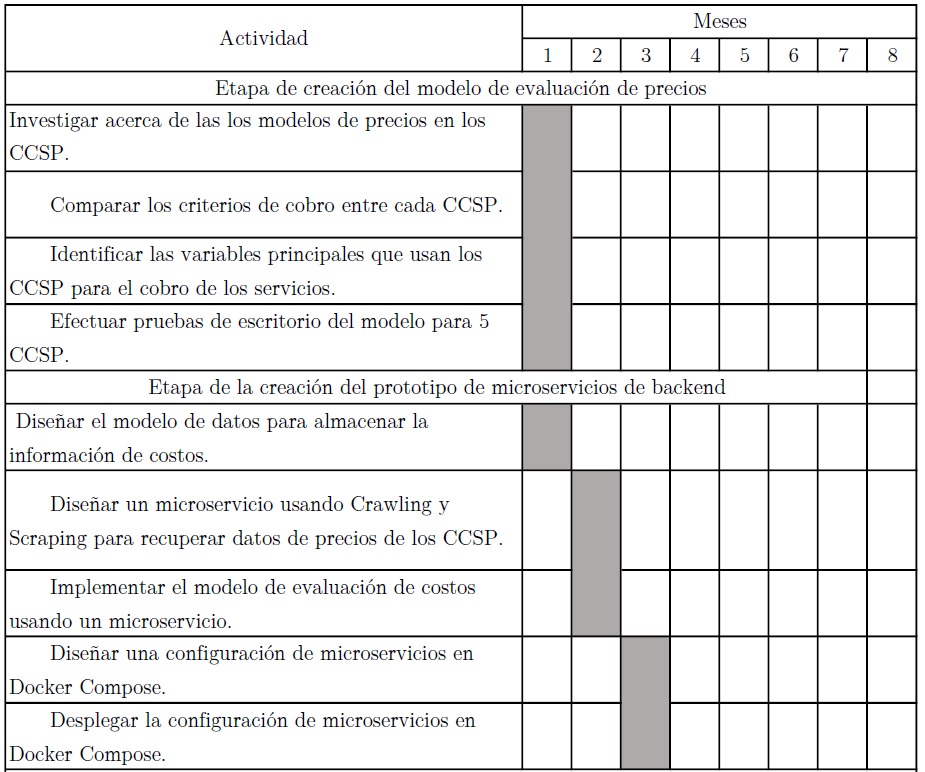
\includegraphics[width=\textwidth]{gfx/actividades.png}
\end{center}

\section{1er Objetivo específico.}
Las actividades de este objetivo específico tienen como propósito \emph{definir un modelo general de evaluación de costos para el análisis de los servicios en el \acrshort{CC} usando información recuperable y relevante de la Web de sus proveedores.} El resultado obtenido son las ecuaciones del modelo de evaluación de costos listas para implementación. A continuación el resumen de cada actividad.

\subsection{Actividad 1.}
Investigar acerca de las los modelos de precios en los \acrshortpl{CCSP}.

\subsection{Actividad 2.}
Comparar los criterios de cobro entre cada \acrshort{CCSP}.

\subsection{Actividad 3.}
Identificar las variables principales que usan los \acrshortpl{CCSP} para el cobro de los servicios.

\subsection{Actividad 4.}
Efectuar pruebas de escritorio del modelo para 5 \acrshortpl{CCSP}.

\section{2do Objetivo específico.}
Las actividades de este objetivo específico tienen como propósito \emph{diseñar e implementar un prototipo basado en microservicios que recopile periodicamente y almacene las tarifas de los principales \acrshortpl{CCSP}}. El resultado obtenido es un Web service que desempeña las tareas mencionadas. A continuación el resumen de cada actividad.

\subsection{Actividad 5.}
Diseñar el modelo de datos para almacenar la información de costos.

\subsection{Actividad 6.}
Diseñar un microservicio que use técnicas de \emph{Crawling} y \emph{Scraping} para recuperar datos de precios de los \acrshortpl{CCSP}.

\subsection{Actividad 7.}
Implementar el modelo de evaluación de costos usando un microservicio.

\subsection{Actividad 8.}
Diseñar una configuración de microservicios en \gls{Docker Compose}.

\subsection{Actividad 9.}
Desplegar la configuración de microservicios en \gls{Docker Compose}.


\newpage

%----------------------------------------------------------------------------------------
